\chapter{CFD Analysis}\label{cp:cfd}

\section{Aerodynamic Performance Curves}\label{sec:aero_perf_curves}

\subsection{Configuration}\label{ssec:configuration}

After our \acrshort{cad} model without the tail was completed, we imported it into the STAR-CCM+ template provided on Canvas. Then, we followed the instructions given to us and set up our solid aircraft body. The only numerical inputs we provided Star-CCM+ were our cruise altitude (\qty{1500}{ft}) and our cruise free stream velocity (\qty{40}{MPH}). After this, a job was submitted to the \acrfull{hpc} cluster to iterate through our solution for the forces acting on the aircraft at an \acrfull{aoa} sweep of \qtyrange{-5}{10}{\degree}. 

Our \acrshort{cad} team had created a model of our aircraft with a tail, but our flight performance team wanted to only do our \acrfull{cfd} analysis with the fuselage and airfoil and use those results for our proper tail sizing if changes were needed.

We were also provided with an Excel sheet to facilitate the calculation of our full-body data given the data from our aircraft model without the tail. As inputs, we used the same free stream velocity and altitude, as well as adding our wingspan (\qty{85}{in}) and our planform area (\qty{4.72}{ft^2}). 

\newpage

\subsection{Results}\label{ssec:results}

The results from the Excel analysis are shown in \autoref{fig:excel_results}. The velocity field generated from STAR-CCM+ is shown in \autoref{fig:star-ccm+_velocity} at two different \acrshort{aoa}.

\begin{figure}[htpb]
    \centering
    \begin{subfigure}{0.49\textwidth}
        \centering
        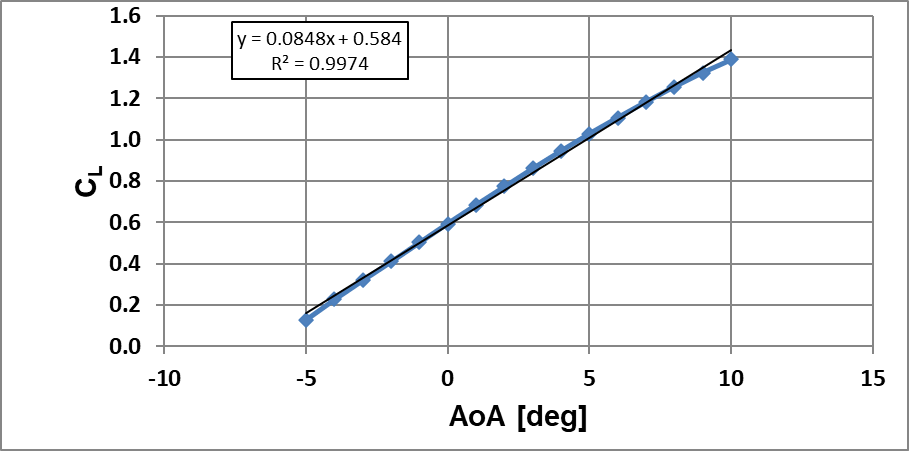
\includegraphics[width=\textwidth]{Figures/cl_vs_aoa.png}
        \caption{Coefficient of lift \gls{C_L} vs. \acrshort{aoa} \gls{alpha}.}
        \label{fig:cl_vs_aoa}
    \end{subfigure}
    \begin{subfigure}{0.49\textwidth}
        \centering
        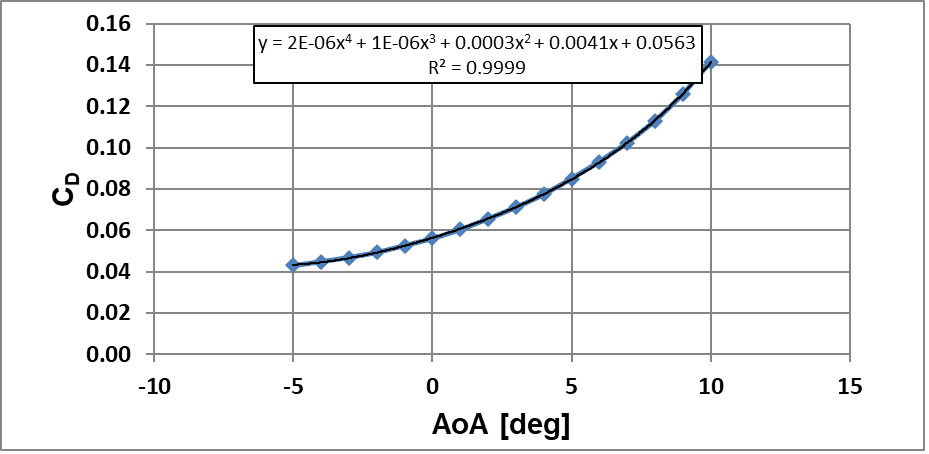
\includegraphics[width=\textwidth]{Figures/cd_vs_aoa.png}
        \caption{Coefficient of drag \gls{C_D} vs. \acrshort{aoa} \gls{alpha}.}
        \label{fig:cd_vs_aoa}
    \end{subfigure} \\
    \begin{subfigure}{0.49\textwidth}
        \centering
        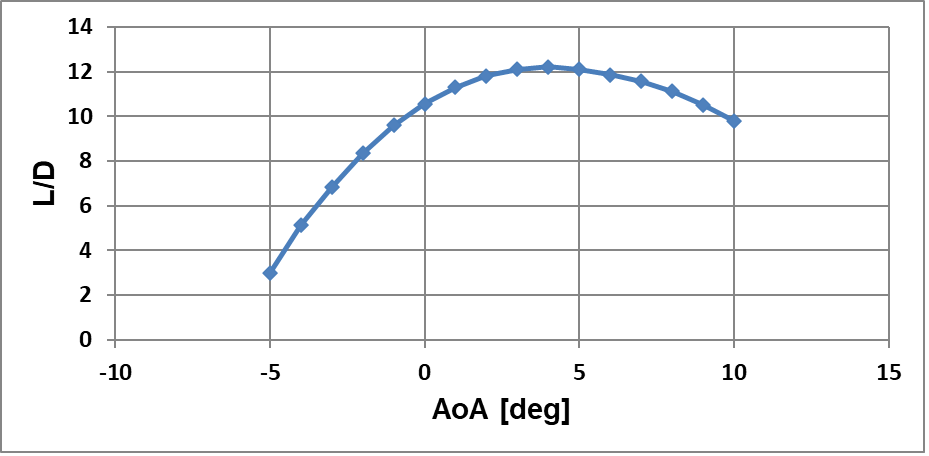
\includegraphics[width=\textwidth]{Figures/ld_vs_aoa.png}
        \caption{Lift-drag ratio \gls{L-by-D} vs. \acrshort{aoa} \gls{alpha}.}
        \label{fig:ld_vs_aoa}
    \end{subfigure}
    \caption[Performance curves from Excel]{Results from the Excel sheet analysis.}
    \label{fig:excel_results}
\end{figure}

\begin{figure}[htpb]
    \centering
    \begin{subfigure}{0.49\textwidth}
        \centering
        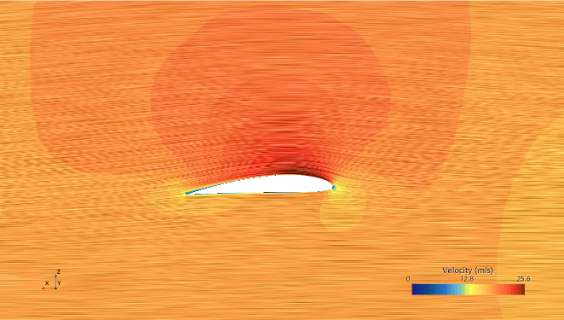
\includegraphics[width=\textwidth]{Figures/v_field_at_aoa_0_deg.png}
        \caption{Velocity field visualized by STAR-CCM+ at an \acrshort{aoa} of \qty{0}{\degree}.}
        \label{fig:v_field_0_deg}
    \end{subfigure}
    \begin{subfigure}{0.49\textwidth}
        \centering
        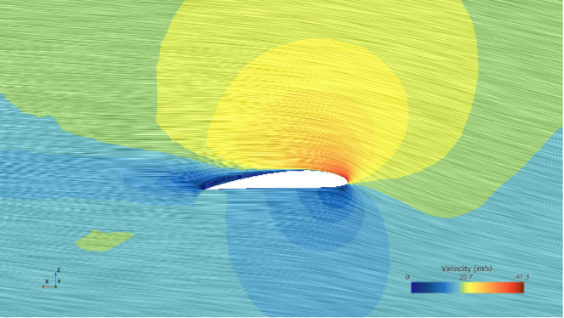
\includegraphics[width=\textwidth]{Figures/v_field_at_aoa_10_deg.png}
        \caption{Velocity field visualized by STAR-CCM+ at an \acrshort{aoa} of \qty{10}{\degree}.}
        \label{fig:v_field_10_deg}
    \end{subfigure}
    \caption[Velocity field from STAR-CCM+]{Velocity fields generated by STAR-CCM+.}
    \label{fig:star-ccm+_velocity}
\end{figure}

\section{Discussion of CFD Results}\label{sec:discussion}

Looking first at \autoref{fig:cl_vs_aoa}, the lift slope is slightly less than our 2D analysis, but overall, our lift coefficient is higher. Our lift coefficient at a \qty{0}{\degree} \acrshort{aoa} is \num{0.6} and our maximum coefficient of list is \num{1.39}, both higher than in our 2D analysis.

From \autoref{fig:cd_vs_aoa}, the maximum \gls{C_D}, based on the maximum \gls{C_L} from \autoref{fig:cl_vs_aoa}, is \num{0.14}, which is much higher than our 2D analysis. We expected this due to the shape of our fuselage causing flow separation and contributing significantly to drag at higher \acrshort{aoa}.

Regarding our \gls{L-by-D} ratio, the maximum value shown in \autoref{fig:ld_vs_aoa} is \num{12.2} at a \qty{4}{\degree} \acrshort{aoa}. This is much less than the \gls{L-by-D} ratio we had calculated in our 2D analysis. Regardless, our 3D \gls{L-by-D} ratio is still fairly high. Another positive result is that our \gls{L-by-D} ratio at \qty{0}{\degree} \acrshort{aoa} is \num{10.6}, which means in \acrfull{slf}, we will still have a high \gls{L-by-D} ratio. 

The results of our initial 2D airfoil analysis and our 3D analysis are tabulated next each other in \autoref{tbl:initial_vs_current_values}.

\begin{table}[htpb]
    \centering
    \caption[2D airfoil analysis vs. current analysis]{The results of the initial 2D airfoil analysis vs. our current analysis, where \gls{dC_L-by-dalpha} is the slope of the coefficient of lift versus angle of attack curve, \gls{C_L_alpha0} is the coefficient of lift when the \acrshort{aoa} is zero, \gls{C_L_max} is the maximum value of the coefficient of lift curve, \gls{C_D_max} is the maximum value of the drag coefficient, and \gls{L-by-D_max} is the maximum value of the lift-drag ratio.}
    \begin{tabular}{ccc}
        \toprule
        \textbf{Parameter} & \textbf{2D} & \textbf{3D} \\
        \midrule
        \gls{dC_L-by-dalpha} & \num{0.1} & \num{0.08} \\
        \gls{C_L_alpha0} & \num{0.45} & \num{0.6} \\
        \gls{C_L_max} & \num{1.31} & \num{1.39} \\
        \gls{C_D_max} & \num{0.078} & \num{0.14} \\
        \gls{L-by-D_max} & \num{19.3} & \num{12.2} \\
        \bottomrule
    \end{tabular}
    \label{tbl:initial_vs_current_values}
\end{table}

The only concerns we have with our results are regarding our ``Optimized Linear Range for Stability Analysis.'' Our valid linear range was only for negative \acrshort{aoa}, so we may need to investigate why this is occurring before doing stability analysis. This graph was not needed for our preliminary aerodynamic performance analysis but will be important later when sizing our tail components. 

Additionally, we wanted to analyze the velocity vector field of our wing at a \qty{0}{\degree} \acrshort{aoa} and at a \qty{10}{\degree} \acrshort{aoa}. The resulting velocity fields are shown in \autoref{fig:v_field_0_deg} and \autoref{fig:v_field_10_deg}. We found that because the \acrshort{naca} 4412 is a thicker airfoil and because our fuselage has significant flow separation, there is a large wake of low velocity flow at higher \acrshort{aoa}. This is important to remember for our tail design.

\section{Future Improvements}\label{sec:future_improvements}

Overall, our results from the STAR-CCM+ \acrshort{cfd} analysis were good for our mission. Our \gls{L-by-D} ratios are less than expected compared to our 2D analysis, but they are still relatively high and are expected to be good for maximizing our loiter time. Our maximum lift coefficient is higher than expected, which is desirable for maximizing our lift force. Our flight performance sub team does not believe any major design changes need to be made.

The only major improvements to our design we are considering is changing our fuselage shape or our wing position. Making the back of our fuselage more streamlined and flushed with the tail spar would reduce flow separation and improve the velocity of the flow that reaches the tail. If we cannot change the fuselage shape, it may be worthwhile to consider changing the position of our main wing to a shoulder-mounted position. Regardless, more analysis needs to go into our wake profile before those considerations are acted upon.

\section{CFD File References}\label{sec:file_ref}

The results of our \acrshort{cfd} analysis are located in the shared CyBox folder under the \verb|2024-10-04_PreliminaryCFD_AirfoilFuselage| directory with the following file names:

\begin{itemize}
    \item \verb|461-AirfoilFuselageCFD@06000.sim| - STAR-CCM+ simulation file at \num{6000} iterations
    \item \verb|461-AirfoilFuselageCFD@22000.sim| - STAR-CCM+ final simulation file
    \item \verb|AirfoilFuselage_ForceAndMomentEvery1000.csv| - force and moment data from STAR-CCM+
    \item \verb|CFD_AirfoilFuselage_Data.xlsm| - the provided analysis template from Canvas
\end{itemize}
